\chapter{Metodologia}
\label{cap:03}

Nesta seção, serão apresentados os materiais e métodos utilizados no estudo, detalhando a metodologia adotada e os procedimentos experimentais realizados. O processo inicia com o levantamento de dados necessários para a análise e estudo, seguido de uma avaliação criteriosa dos processos envolvidos. Com base nessas análises, será estruturado o desenvolvimento do trabalho, garantindo que todas as etapas sejam realizadas de forma sistemática e alinhadas aos objetivos do projeto.

Serão discutidos os principais passos estabelecidos para a execução completa do projeto idealizado, conforme ilustrado na Figura \ref{fig:desenvolvimento}.

\begin{figure}[ht]
    \caption{Diagrama dos passos para a conclusão da ferramenta}
    \centering
    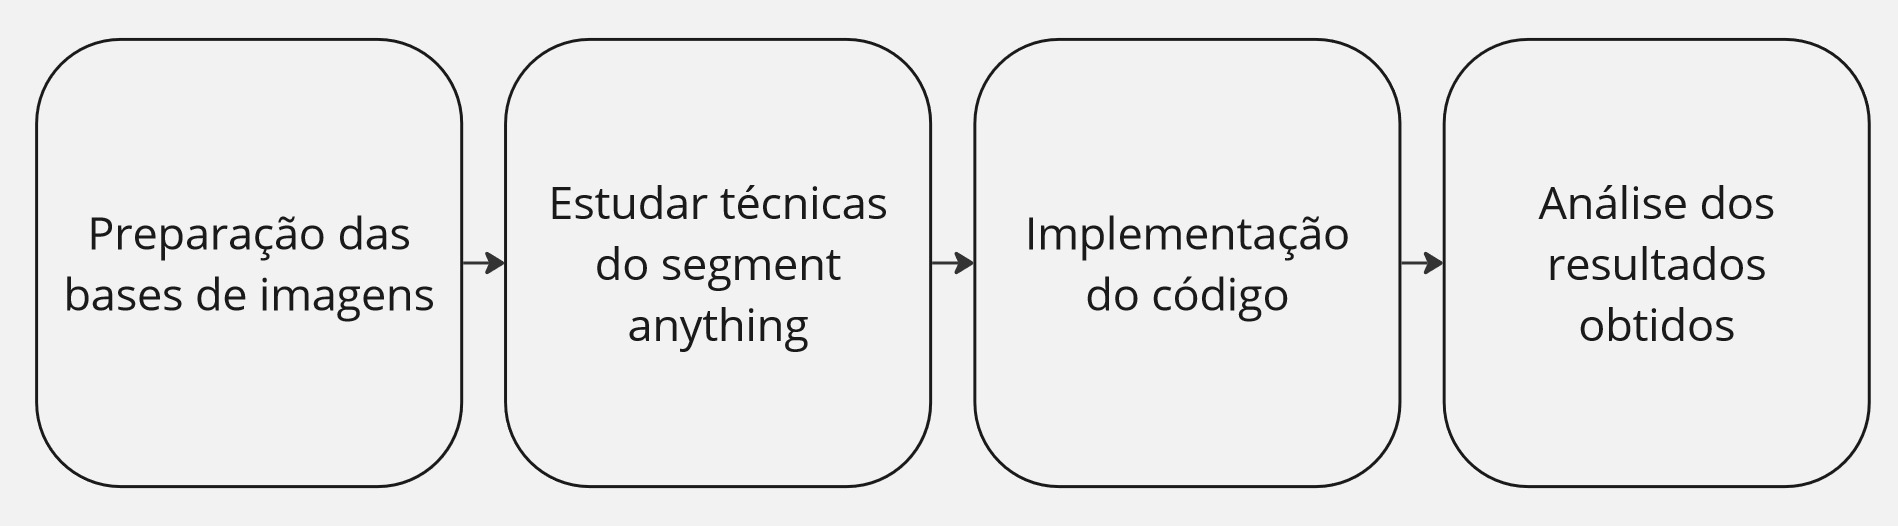
\includegraphics[scale=0.2]{imagens/progresso_desenvolvimento.jpg}

    Fonte: Elaborado pelo autor
    \label{fig:desenvolvimento}
\end{figure}

O diagrama apresentado acima aborda os passos necessários para a realização da segmentação de imagem

A realização da segmentação de imagem é um processo complexo que envolve várias etapas importantes como foi mostrado o diagrama na Figura \ref{fig:desenvolvimento}. Uma das principais técnicas utilizadas atualmente é o Zero-Shot, que permite às inteligências artificiais aprender a segmentar imagens sem a necessidade de exemplos prévios. Isso é possível graças ao uso de modelos de linguagem treinados em grandes conjuntos de dados, que permitem a transferência de conhecimento para novas tarefas como exemplificado por \citeauthorandyear{Cao2022}.

Antes de nos aprofundar nos conceitos do segment Anything é importante mostrar alguns conceitos sobre as técnicas de segmentação usadas, pois existem diversos tipos de segmentação usados por inteligências artificiais, cada um com objetivos e abordagens específicas para a análise de imagens. A segmentação de imagens é essencialmente o processo de dividir uma imagem em diferentes regiões ou segmentos, com base em características como cor, textura ou bordas, para facilitar a análise e o entendimento do conteúdo da imagem. Entre as abordagens mais comuns estão a segmentação semântica, a segmentação instanciada e a segmentação baseada em objetos.

A segmentação semântica é o processo em que cada pixel da imagem é classificado em uma categoria específica, como céu, água, chão, etc. Esse tipo de segmentação não diferencia as instâncias de objetos dentro de uma mesma categoria. Por exemplo, em uma imagem de um campo com várias árvores, todas as árvores seriam tratadas como um único objeto, sem distinção entre elas.

Já a segmentação instanciada vai além, separando as diferentes instâncias de um mesmo tipo de objeto. Ou seja, mesmo que uma imagem contenha múltiplas árvores, a IA seria capaz de distinguir uma árvore da outra, tratando-as como objetos individuais. Esse tipo de segmentação é crucial para tarefas que exigem uma compreensão mais detalhada da cena, como a análise de objetos em vídeos ou imagens complexas.

A segmentação baseada em objetos, por sua vez, foca na identificação e separação dos objetos em uma imagem com base em suas características visuais. Diferentemente da segmentação semântica, que classifica pixels de maneira geral, a segmentação baseada em objetos busca identificar e delimitar objetos específicos dentro da cena, como pessoas, veículos ou animais. Esse tipo de segmentação é frequentemente utilizado em sistemas de visão computacional para tarefas como reconhecimento de objetos, detecção e rastreamento.

Essas técnicas de segmentação são utilizadas em conjunto com modelos avançados de aprendizado de máquina, como o Segment Anything Model (SAM), que aproveita grandes bases de dados e métodos como o Zero-Shot Learning para adaptar seus algoritmos a novos tipos de imagens e cenários. Cada uma dessas abordagens tem sua aplicação dependendo do tipo de tarefa a ser realizada e das necessidades do projeto, com a segmentação instanciada e a baseada em objetos oferecendo uma compreensão mais detalhada e precisa dos elementos presentes nas imagens.

Um exemplo de modelo que utiliza essa técnica é o Segment Anything, que foi treinado em uma base de 11 milhões de imagens\footnote{informações obtidas através do link: https://ai.meta.com/datasets/segment-anything/}. Essa base é composta por imagens que tem a média de resolução de 1500×2250. Além disso, o Segment Anything também foi treinado em diferentes tipos de imagens, incluindo objetos, cenas e ações, o que o torna um modelo versátil e capaz de lidar com diferentes tipos de segmentação.

No entanto, criar uma base de imagens própria para treinar um modelo de segmentação pode ser um trabalho manual imenso. Isso é especialmente verdadeiro quando se trata de pixel art, pois não foi encontrada nenhuma base de dados pública que contenha imagens desse tipo já segmentada. Portanto, seria necessário criar uma base de imagens do zero, o que exigiria um grande esforço e tempo.

Diante disso, as etapas para realizar a segmentação de imagem podem ser resumidas da seguinte forma: em primeiro lugar, é necessário preparar as bases de imagens, o que pode envolver a criação de uma base própria como o caso deste trabalho, com 50 pixel artes de diferentes resoluções e cenas. Em seguida, é importante estudar as técnicas utilizadas pelo Segment Anything e outros modelos de segmentação, para entender como eles funcionam e como podem ser adaptados para a tarefa específica.

Após isso, é necessário implementar o código para testar o modelo de segmentação. Isso deve envolver a utilização de bibliotecas de aprendizado de máquina. Por fim, é importante analisar os resultados obtidos, para avaliar a eficácia do modelo e identificar áreas para melhoria.

Em resumo, a segmentação de imagem é um processo complexo que envolve várias etapas importantes, desde a preparação das bases de imagens até a análise dos resultados obtidos. A utilização de técnicas de Zero-Shot e modelos como o Segment Anything deve facilitar o processo, mas ainda é necessário um grande esforço e tempo para criar uma base de imagens próprias para a comparação com os resultados gerados pela inteligencia artificial.


\section{Tecnologias utilizadas}
Nesta seção, será abordado sobre as diferentes bibliotecas estudadas para que a análise pudesse ser feita com o melhor aproveitamento da linguagem.
será mostrado também alguns tópicos referente ao estudo do python como linguagem em geral.

Para a criação da ferramenta de análise será utilizado o ambiente de desenvolvimento Visual Studio Code utilizando Python, foi optado este ambiente por sua praticidade com os diversos formatos de arquivos que serão utilizados ao decorrer do projeto. 
O python também servirá como única linguagem de programação para a facilidade com a criação e uso das bibliotecas de inteligencia Artificial que irá adiantar muitos dos processos necessários para a criação da análise.

Para iniciar o estudo das bibliotecas antes, deve se entender melhor sobre os ambientes do python como o ambiente virtual, além de estudar como é o funcionamento das IDEs com o ambiente python dá mesma forma.

\begin{itemize}
    \item \textbf{PyTorch:}  
    Para o uso do \textit{SegmentAnything}, o \textit{PyTorch} é uma das dependências cruciais, já que ele aborda todo o processamento usado por placas de vídeo e sistemas integrados com maior facilidade. O estudo dessa biblioteca se faz necessário apenas para a instalação de seus softwares dependentes, como o uso do NVIDIA CUDA, entre outros sistemas terceiros, para o funcionamento do \textit{Segment Anything}.

    \item \textbf{Scikit-image:}  
    O \textit{Scikit-image} será extremamente necessário para a análise dos recursos e resultados obtidos, pois é com ele que conseguimos facilmente gerar as estatísticas como o MSE, por exemplo. Não apenas isso, mas o estudo dessa ferramenta deve vir análogo ao estudo dos métodos de estimativa comparando duas imagens.

    \item \textbf{OpenCV:}  
    O OpenCV (\texttt{cv2}) será empregado para lidar com tarefas relacionadas ao processamento de imagens, como leitura, conversão e redimensionamento. Ele será utilizado para ler as imagens a partir do disco (\texttt{cv2.imread}) e convertê-las entre diferentes espaços de cores para garantir a consistência de dados durante o processamento. Por exemplo, a função \texttt{cv2.cvtColor} será usada para converter as imagens do formato BGR para RGB, alinhando-as ao formato de cores esperado pelo modelo de segmentação. Além disso, o OpenCV será usado para redimensionar as imagens (\texttt{cv2.resize}) a fim de assegurar que elas possuam o mesmo tamanho antes de realizar comparações e cálculos de correlação. Um dos métodos-chave será o cálculo da Correlação Cruzada Normalizada (NCC), que será realizado por meio da função \texttt{cv2.matchTemplate}. Esse método permitirá medir a similaridade entre a imagem segmentada e a imagem esperada, fornecendo uma métrica quantitativa para avaliar a precisão do processo de segmentação.

    \item \textbf{Numpy:}  
    No projeto, o \texttt{numpy} será fundamental para a manipulação eficiente de arrays multidimensionais, que representarão as imagens processadas. O \texttt{numpy} será utilizado para criar e gerenciar esses arrays, facilitando a realização de operações matemáticas e comparações pixel a pixel nas imagens. Por exemplo, a função \texttt{np.zeros} será utilizada para inicializar uma matriz de zeros que servirá como base para a imagem segmentada final na função de geração de máscara. Além disso, o \texttt{numpy} permitirá a execução de operações eficientes, como a comparação entre arrays de imagens para verificar a igualdade de pixels com a função \texttt{np.array\_equal}. As imagens serão normalizadas convertendo os valores de pixel para um formato de ponto flutuante, possibilitando uma análise mais precisa ao dividir os valores por 255.0.
\end{itemize}

\section{Procedimentos e técnicas}

Para o desenvolvimento desta pesquisa, foram realizados testes preliminares explorando toda a capacidade do modelo Segment Anything (SAM), com o intuito de validar a eficácia dos processos envolvidos na análise de segmentação de imagens. Durante essa fase inicial, foi constatado que o tempo de processamento se mostrou elevado, mesmo em um sistema com hardware moderno. Como resultado, optou-se por não utilizar a tecnologia NVIDIA CUDA, uma vez que o uso intensivo de processamento pela GPU não seria imprescindível para o escopo do projeto.

Com essa decisão tomada, iniciou-se uma nova bateria de testes envolvendo diferentes tipos de imagens, abrangendo diversas categorias visuais, a fim de avaliar o potencial de segmentação do SAM em variados contextos. Os resultados foram, em sua maioria, satisfatórios, com o modelo demonstrando desempenho adequado na maioria dos casos analisados.

Posteriormente, iniciou-se o desenvolvimento de imagens específicas, criadas pelo autor em estilo pixel art, para validar a performance do modelo em situações de segmentação por cor. Essa etapa exigiu ajustes no código, especialmente no que diz respeito à manipulação das camadas e formatos das imagens, além da tipagem adequada em Python. Esse processo envolveu pesquisas extensivas e múltiplas tentativas até a obtenção de um resultado satisfatório na geração de grupos de cores a partir das imagens.

Com o sistema de segmentação de imagens em funcionamento, iniciou-se a etapa de criação manual das camadas de segmentação. O autor definiu como deveriam ser os resultados esperados da segmentação proposta pela IA, segmentando um conjunto de 50 imagens em estilo pixel art com base em cores específicas para realizar as análises. A partir desse ponto, foi possível aplicar métodos existentes para a comparação entre duas imagens.

Inicialmente, foi desenvolvido um método dentro do código em python para validar a quantidade de pixels corretos, esse algoritmo inicialmente no pixel 0x0 ele gera uma conexão entre a cor original e a cor esperada, assim ele segue até o final da imagem, se caso ele encontrar uma cor diferente no original ele gera um erro, se não ele prossegue assim ele pode calcular com uma boa margem, já que quando se fala de pixel arte, onde a amplitude entre as cores é maior. 

\subsection{Base de dados}

A seleção de uma base de imagens adequada é um passo fundamental para a realização de experimentos em visão computacional, especialmente em estudos que envolvem segmentação de imagens. Neste trabalho, foi utilizada uma base de imagens composta por amostras de média e baixa resolução, com o objetivo de avaliar a eficácia do modelo Segment Anything (SAM) em diferentes contextos de qualidade visual.

As imagens foram escolhidas de modo a abranger uma variedade de cenários, incluindo personagens, cenários, estruturas e objetos, a fim de garantir a representatividade e a diversidade dos dados. Além disso, as resoluções das imagens variaram entre 32x32 \textit{pixels} e 176x256, permitindo uma análise comparativa detalhada do desempenho do SAM em diferentes cenários de pixel arte.

A base foi composta por imagens próprias e conjuntos de imagens gratuitas da plataforma Itch.io\footnote{Acesso através do link: https://itch.io/}, para assegurar a consistência nos experimentos, todas as imagens passaram por um pré-processamento, que incluiu segmentar manualmente todas as imagens. Esse processo foi essencial para padronizar os dados e minimizar a interferência de variáveis externas que pudessem comprometer a análise dos resultados.

A seguir será apresentado algumas das imagens da base para uma melhor definição dos cenários obtidos na análise como na Figura \ref{fig:base_dados_1}.

\begin{figure}[ht]
    \caption{Imagem de exemplo original}
    \centering
    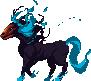
\includegraphics[scale=2]{imagens/nightmare-idle.png}

    Fonte: https://itch.io/
    \label{fig:base_dados_1}
\end{figure}

E após a segmentação manual, temos a seguinte imagem, lembrando que alguns padrões de cores foram utilizados para que fosse mais fácil identificar e comparar com os dados vindos do (SAM).

\begin{figure}[ht]
    \caption{Imagem de exemplo pós segmentação manual}
    \centering
    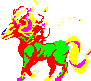
\includegraphics[scale=2]{imagens/nightmare-idle-v2.png}

    Fonte: Elaborado pelo autor
    \label{fig:base_dados_2}
\end{figure}

Já na Figura \ref{fig:base_dados_2}, podemos ver cores bem fortes mostrando qual deveria ser a mascara realizada para a comparação futura.

\section{Métricas Utilizadas}

Para avaliar a qualidade dos resultados obtidos, foram utilizadas duas métricas amplamente conhecidas na área de visão computacional: o \textit{Erro Médio Quadrático (Mean Squared Error - MSE)} e a \textit{Correlação Cruzada Normalizada (Normalized Cross-Correlation - NCC)}. Abaixo, são descritas as fórmulas e os algoritmos utilizados para o cálculo dessas métricas.

\begin{itemize}
    \item \textbf{Erro Médio Quadrático} \\
    O MSE mede a diferença média ao quadrado entre os valores previstos e os valores reais, sendo uma métrica que avalia o erro absoluto entre a segmentação obtida e a referência. Quanto menor o valor do MSE, mais próximo o resultado está do esperado. A fórmula do MSE é dada por:

    \[
    MSE = \frac{1}{N} \sum_{i=1}^{N} (x_i - y_i)^2
    \]

    Onde:
    \begin{itemize}
        \item \( x_i \): Valor previsto (ou resultado da segmentação).
        \item \( y_i \): Valor real (ou referência).
        \item \( N \): Número total de pixels na imagem.
    \end{itemize}

    \item \textbf{Correlação Cruzada Normalizada} \\
    
    A Correlação Cruzada Normalizada (NCC) é uma métrica amplamente utilizada no processamento de imagens para medir a similaridade estrutural entre duas imagens. Diferentemente de outras métricas, como o Erro Médio Quadrático (MSE), a NCC considera a relação de intensidade entre os pixels de ambas as imagens, desconsiderando variações de escala ou deslocamento que possam ocorrer. O valor da NCC é normalizado, variando entre -1 e 1. Um valor de NCC igual a 1 indica que as imagens são estruturalmente idênticas, ou seja, há uma correspondência perfeita entre seus pixels. Por outro lado, um valor de NCC igual a -1 reflete uma relação totalmente inversa entre as imagens, em que uma é o negativo estrutural da outra. Quando a NCC está próxima de 0, isso sugere uma baixa correlação, indicando pouca ou nenhuma semelhança estrutural entre as imagens.

    A fórmula para calcular a NCC utiliza a média e os valores de intensidade dos pixels das duas imagens, considerando a soma ponderada das diferenças entre os valores individuais de cada pixel e suas respectivas médias. Por ser uma métrica normalizada, a NCC é especialmente robusta contra alterações de brilho ou contraste, concentrando-se apenas na estrutura relativa das imagens. Essa característica faz com que a NCC seja amplamente empregada em tarefas como registro de imagens, rastreamento de objetos e detecção de padrões, onde a identificação precisa de semelhanças estruturais é essencial.Sua fórmula é dada por:

    \[
    NCC = \frac{\sum_{i=1}^{N} (x_i - \bar{x})(y_i - \bar{y})}{\sqrt{\sum_{i=1}^{N} (x_i - \bar{x})^2 \cdot \sum_{i=1}^{N} (y_i - \bar{y})^2}}
    \]

    Onde:
    \begin{itemize}
        \item \( x_i \): Valor de intensidade do pixel na imagem segmentada.
        \item \( y_i \): Valor de intensidade do pixel na imagem de referência.
        \item \( \bar{x} \): Média dos valores dos pixels na imagem segmentada.
        \item \( \bar{y} \): Média dos valores dos pixels na imagem de referência.
    \end{itemize}
\end{itemize}